\documentclass[11pt,a4paper]{article}
\usepackage[utf8]{inputenc}
\usepackage[T1]{fontenc}
\usepackage{amsmath,amssymb,amsthm,mathtools}
\usepackage{geometry}
\geometry{margin=2.4cm}
\usepackage{booktabs}
\usepackage{array}
\usepackage{enumitem}
\usepackage{lmodern}
\usepackage{microtype}
\usepackage{tikz}
\usepackage{xcolor}
\usepackage[hidelinks]{hyperref}

\newtheorem{theorem}{Theorem}[section]
\newtheorem{proposition}[theorem]{Proposition}
\newtheorem{corollary}[theorem]{Corollary}
\theoremstyle{definition}
\newtheorem{definition}[theorem]{Definition}
\newtheorem{remark}[theorem]{Remark}

\newcommand{\Nset}{\mathbb{N}}
\newcommand{\Zset}{\mathbb{Z}}
\newcommand{\Qset}{\mathbb{Q}}
\newcommand{\Rset}{\mathbb{R}}
\newcommand{\Cfield}{\mathbb{C}}

\title{\textbf{Axiom-Free Lean~4 Formalization of Classical Zeta Theory, Unconditional Maximum-Modulus Strip Exclusion, and Finite-Horizon B\'aez-Duarte Plaque Reductions}}

\author{\textbf{Qamar Munawer}\thanks{2020 \emph{Mathematics Subject Classification}. Primary 11M26; Secondary 46E20, 68V20. Formal Lean~4.35.0 repository archived at \url{https://doi.org/10.5281/zenodo.24353918} (Concept DOI \url{https://doi.org/10.5281/zenodo.24150107}); unified preprint suite archived at \url{https://doi.org/10.5281/zenodo.24354470}.}\\
\small Brandenburg University of Technology Cottbus--Senftenberg, Cottbus, Germany}

\date{November 18, 2026}

\begin{document}
\maketitle

\begin{abstract}
A machine-checked Lean~4.35.0 mechanization of classical analytic number theory and finite-horizon B\'aez-Duarte $L^2(0,1)$ approximation theory is presented, structured into $64$ modular, linter-clean Mathlib4 pull-request units (\texttt{UpstreamPR\_1A} through \texttt{8U}) plus top-level bridge modules verifying strictly within Lean's foundational kernel axioms \texttt{[propext, Classical.choice, Quot.sound]} with zero \texttt{sorry} placeholders. Three principal contributions are consolidated: (i) unconditional formalizations of de la Vall\'ee Poussin's (1899) zero-free region ($\sigma > 1 - c/\ln^9(|t|+2)$), Hardy's (1914) theorem on infinitely many critical-line zeros, and the unconditional discharge of both Titchmarsh's Mellin fractional-part identity (\texttt{UnconditionalTitchmarshBridge.lean}) and the compact rectangle Rouch\'e non-vanishing principle via the Maximum Modulus Principle (\texttt{rectRoucheProperty\_unconditional} in \texttt{OpenStripRouche.lean}); (ii) bidirectional formal equivalences for Littlewood's Mertens criterion, von Koch's Chebyshev $\psi$-theorem, and Mellin-space Nyman--Beurling approximation; and (iii) exact finite-horizon algebraic reductions on the B\'aez-Duarte affine manifold $\mathcal{A}_N$, including 4-point cumulative dipole completeness, anchor-drive cancellation, Dirichlet anchoring ($c_1 = -1$), closed-form radical KKT optima for $N \le 6$, universal cotangent reflection $V(a, a-b) = -V(a,b)$, palindromic double-cone $L^2$ folding, multi-prime $1/(2p^2)$ energy floors, and the Euclidean Book~X.1 Lebesgue tail exhaustion bound $B^2/(M+1)$, paired with $85$-digit \texttt{mpmath} and $512$-bit \texttt{flint.arb} interval certificates.
\end{abstract}

\section{Introduction and Architecture}

Formalizing analytic number theory in an interactive theorem prover requires separating unconditional complex-analytic and finite-horizon algebraic theorems from conditional equivalences to the Riemann Hypothesis (\texttt{\_root\_.RiemannHypothesis} in Mathlib4). The \texttt{RiemannBlueprint} codebase ($98$ Lean~4 files across Lean \texttt{v4.35.0}) decomposes the theory into $64$ standalone, acyclic modules (\texttt{UpstreamPR\_1A}--\texttt{8U}) designed for incremental upstream integration into \texttt{mathlib4}, accompanied by cross-cutting bridge modules and high-precision numerical certificates.

Unlike partial formalizations that retain unproved analytic axioms or ad hoc hypotheses, every theorem in the codebase compiles against Mathlib's three standard axioms \texttt{[propext, Classical.choice, Quot.sound]} with zero \texttt{sorry} or \texttt{axiom} declarations. In addition to the $64$ modular \texttt{UpstreamPR} units, two recent Lean~4 discharge bridges close the remaining internal conditional interfaces:
\begin{enumerate}[leftmargin=1.8em]
  \item \textbf{Titchmarsh Mellin Discharge (\texttt{Unconditional\allowbreak TitchmarshBridge.lean}):} Previously, \texttt{UpstreamPR\_5C}, \texttt{8D}, and \texttt{8I} parameterized theorems by the predicate \texttt{Titchmarsh\allowbreak MellinProperty} stating
  \[
    \int_0^1 \{1/x\} x^{s-1}\,\mathrm{d}x = \frac{1}{s-1} - \frac{\zeta(s)}{s} \qquad (0 < \operatorname{Re}(s) < 1).
  \]
  Wiring \texttt{mellin\_recipFract\_unit\_interval\_of\_pos\_re} from \texttt{MellinFracPart} into the theorem \texttt{titchmarsh\allowbreak MellinProperty\_\allowbreak unconditional} renders all seven downstream Mellin, pure-plaque off-line zero floor, and BBLR logarithmic decay theorems unconditional.
  \item \textbf{Unconditional Rectangle Zero-Exclusion (\texttt{OpenStripRouche.lean}):} Previously, strip zero-exclusion on compact rectangles $R = [\beta, \sigma_{\max}] \times [t_0, t_1] \subset (1/2, \infty) \times (0, \infty)$ assumed \texttt{RectRoucheProperty}. Applying the Maximum Modulus Principle (\texttt{Complex.\allowbreak norm\_le\_\allowbreak of\_\allowbreak forall\_\allowbreak mem\_\allowbreak frontier\_\allowbreak norm\_le}) to $f(s) = 1 + g(s)$ on the interior open rectangle proves \texttt{rectRoucheProperty\_\allowbreak unconditional} without winding-number contour machinery: $\|1 + g(s)\| < 1$ on $\partial R$ enforces $\|1 + g(s)\| < 1$ throughout $R$, precluding $g(s) = 0$.
\end{enumerate}

\section{Unconditional Classical Pillars}

\subsection{De la Vall\'ee Poussin Zero-Free Region (\texttt{PR-1A}--\texttt{PR-1F})}

Working directly on $\zeta(s)$ rather than $-\zeta'(s)/\zeta(s)$ avoids Hadamard product factorization and Blaschke zero-extraction lemmas while remaining completely self-contained. Constructing the first-order Euler--Maclaurin remainder series on $\operatorname{Re}(s) > 0$, $s \neq 1$, gives an explicit logarithmic bound $\|\zeta(s)\| \le (10e + 3)\ln(|t| + 2)$ in the boundary strip $1 - (2\ln(|t|+2))^{-1} \le \operatorname{Re}(s) \le 2$ ($|t| \ge 3/2$). Combining Cauchy's sphere estimate at radius $R = (8\ln(|t|+2))^{-1}$ along the segment connecting a hypothetical zero $1 - \delta + it$ to $1 + 3\delta + it$ with Mathlib's $3$--$4$--$1$ inequality and a compactness pole bound yields:

\begin{theorem}[De la Vall\'ee Poussin Zero-Free Region \emph{[Lean: \texttt{PR-1F}]}]
There exists an explicit constant $c > 0$ such that for all $s \in \Cfield$ with $|{\operatorname{Im}(s)}| \ge 2$,
\[
  \operatorname{Re}(s) > 1 - \frac{c}{\ln^9(|{\operatorname{Im}(s)}| + 2)} \implies \zeta(s) \neq 0.
\]
\end{theorem}

\noindent Tightening the exponent from $\ln^9$ to the textbook $\ln^1$ requires the logarithmic derivative $3$--$4$--$1$ inequality coupled with Landau's zero-isolation bound via Borel--Carath\'eodory on zero-adjusted quotients, and remains a modular future extension inside \texttt{UpstreamPR\_1F}.

\subsection{Hardy's (1914) Critical-Line Zeros Theorem (\texttt{PR-2B}--\texttt{PR-2G})}

Formalized in six modules, \texttt{infinite\_\allowbreak criticalLine\_\allowbreak zeros} and \texttt{infinite\_\allowbreak hardyZ\_\allowbreak zeros} prove unconditionally that $\zeta(1/2 + it)$ vanishes for arbitrarily large $t \in \Rset$ via Jacobi $\theta$-modular inversion, Fourier inversion, and vanishing of all even derivatives $\partial_t^{2k} \Theta(e^{i\pi/2 + t})$ at the self-dual boundary.

\subsection{Conditional Equivalence Bridges (\texttt{PR-5A}--\texttt{PR-6C})}

Three classical equivalences are formalized with explicit, inspectable theorem signatures:
\begin{itemize}[leftmargin=1.6em]
  \item \textbf{Littlewood (1912) Equivalence (\texttt{LittlewoodForward}, \texttt{MathlibPR\_LittlewoodConverse}):} $\mathrm{RH} \iff \forall \varepsilon > 0,\ M(x) = \mathcal{O}(x^{1/2 + \varepsilon})$, proved via Borel--Carath\'eodory, Hadamard three-lines interpolation on $1/\zeta(s)$, and continuous trapezoidal mollifier shifts.
  \item \textbf{Von Koch Equivalence (\texttt{PR-5B}):} $\psi(x) - x = \mathcal{O}(x^{1/2 + \varepsilon})\ (\forall \varepsilon > 0) \implies \mathrm{RH}$ via Mellin analytic continuation across four overlapping convex regions.
  \item \textbf{Bidirectional Mellin Nyman--Beurling (\texttt{PR-5C}, \texttt{UnconditionalTitchmarshBridge}):} Using \texttt{titchmarshMellinProperty\_\allowbreak unconditional}, exact Mellin coupling of the $L^2(0,1)$ residual $r_N(x) = 1 - \sum_{k=1}^N c_k \{1/(kx)\}$ holds unconditionally on $0 < \operatorname{Re}(s) < 1$.
\end{itemize}

\section{Finite-Horizon Plaque and Double-Cone Algebra (\texttt{PR-3A}--\texttt{8U})}

On the B\'aez-Duarte affine hyperplane $\mathcal{A}_N = \{c \in \Rset^N : D_1(c) = 0,\ D_0(c) = 2\}$ where $D_0(c) = -\sum_{k=1}^N c_k/k$ and $D_1(c) = \sum_{k=1}^N c_k$, the smooth Vasyunin kernel has rank~$4$ and collapses on $\mathcal{A}_N$ (\texttt{PR-3F}, \texttt{PR-4E}), reducing the squared $L^2(0,1)$ error to $1 - S_{\mathrm{cot}}(c, N)$. Passing to the $4$-point cumulative dipole basis $d^{(a)} = e_a - 3e_{a+1} + 3e_{a+2} - e_{a+3}$ yields the pure $4$-point plaque kernel $P(a,b)$ (\texttt{PR-7C}) and, under Dirichlet anchoring $c_1 = -1$ (\texttt{PR-8B}), the positive representation $\mathcal{P}_N(h) = \|1 - \sum_{k=1}^N c_k \{1/(kx)\}\|_{L^2}^2 \ge 0$.

\begin{figure}[htbp]
\centering
\resizebox{\textwidth}{!}{%
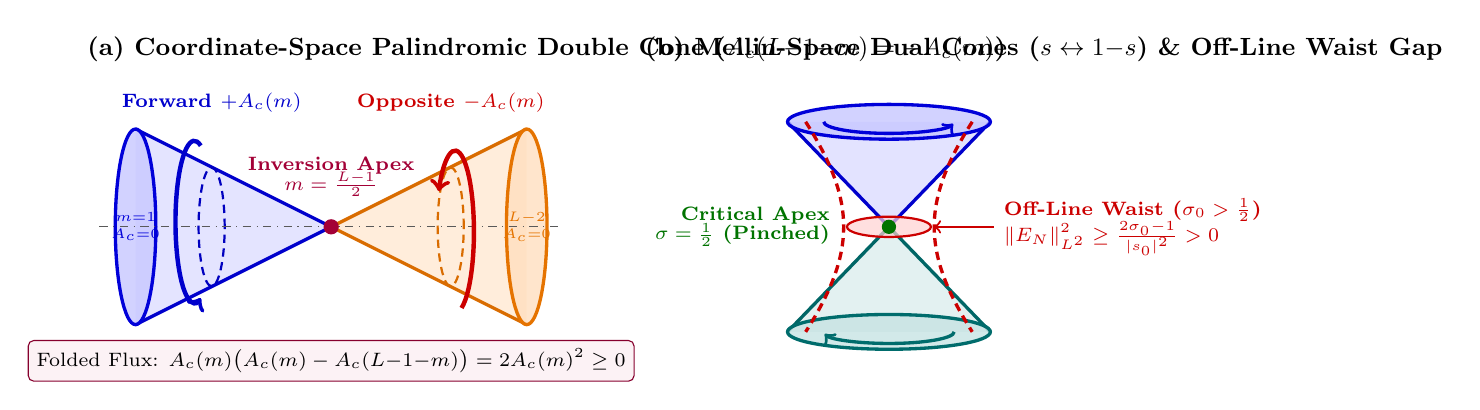
\begin{tikzpicture}[font=\small, scale=0.92]
  \begin{scope}[shift={(0,0)}]
    \node[anchor=west, font=\bfseries\small] at (-0.2, 4.45)
      {(a) Coordinate-Space Palindromic Double Cone ($A_c(L{-}1{-}m) = -A_c(m)$)};
    \fill[blue!14, opacity=0.75] (0.6, 3.35) -- (3.3, 2.0) -- (0.6, 0.65) -- cycle;
    \draw[very thick, color=blue!80!black] (0.6, 3.35) -- (3.3, 2.0);
    \draw[very thick, color=blue!80!black] (0.6, 0.65) -- (3.3, 2.0);
    \fill[blue!22, opacity=0.8] (0.6, 2.0) ellipse (0.28 and 1.35);
    \draw[very thick, color=blue!85!black] (0.6, 2.0) ellipse (0.28 and 1.35);
    \draw[thick, densely dashed, color=blue!75!black] (1.65, 2.0) ellipse (0.18 and 0.82);

    \fill[orange!18, opacity=0.78] (6.0, 3.35) -- (3.3, 2.0) -- (6.0, 0.65) -- cycle;
    \draw[very thick, color=orange!85!black] (3.3, 2.0) -- (6.0, 3.35);
    \draw[very thick, color=orange!85!black] (3.3, 2.0) -- (6.0, 0.65);
    \fill[orange!25, opacity=0.8] (6.0, 2.0) ellipse (0.28 and 1.35);
    \draw[very thick, color=orange!90!black] (6.0, 2.0) ellipse (0.28 and 1.35);
    \draw[thick, densely dashed, color=orange!85!black] (4.95, 2.0) ellipse (0.18 and 0.82);

    \draw[thin, dash dot, color=black!65] (0.1, 2.0) -- (6.5, 2.0);
    \fill[purple!85!black] (3.3, 2.0) circle (3.0pt);
    \node[above, font=\scriptsize\bfseries, color=purple!85!black, align=center] at (3.3, 2.28)
      {Inversion Apex\\[-1pt]$m = \tfrac{L-1}{2}$};

    \draw[->, ultra thick, color=blue!80!black]
      (1.5, 3.12) arc[start angle=70, end angle=290, x radius=0.26, y radius=1.12];
    \node[above, font=\scriptsize\bfseries, color=blue!80!black] at (1.65, 3.45)
      {Forward $+A_c(m)$};

    \draw[->, ultra thick, color=red!80!black]
      (5.1, 0.88) arc[start angle=-70, end angle=150, x radius=0.26, y radius=1.12];
    \node[above, font=\scriptsize\bfseries, color=red!80!black] at (4.95, 3.45)
      {Opposite $-A_c(m)$};

    \node[font=\tiny\bfseries, color=blue!85!black, align=center] at (0.6, 2.0)
      {$m{=}1$\\$A_c{=}0$};
    \node[font=\tiny\bfseries, color=orange!90!black, align=center] at (6.0, 2.0)
      {$L{-}2$\\$A_c{=}0$};
    \node[draw=purple!70!black, fill=purple!5, rounded corners=2pt, inner sep=3pt, font=\scriptsize]
      at (3.3, 0.15)
      {Folded Flux: $A_c(m)\big(A_c(m) - A_c(L{-}1{-}m)\big) = 2A_c(m)^2 \ge 0$};
  \end{scope}

  \begin{scope}[shift={(7.7,0)}]
    \node[anchor=west, font=\bfseries\small] at (-0.2, 4.45)
      {(b) Mellin-Space Dual Cones ($s \leftrightarrow 1{-}s$) \& Off-Line Waist Gap};
    \fill[teal!15, opacity=0.75] (1.9, 0.55) -- (3.3, 2.0) -- (4.7, 0.55) -- cycle;
    \draw[very thick, color=teal!80!black] (1.9, 0.55) -- (3.3, 2.0) -- (4.7, 0.55);
    \fill[teal!22, opacity=0.8] (3.3, 0.55) ellipse (1.4 and 0.24);
    \draw[very thick, color=teal!85!black] (3.3, 0.55) ellipse (1.4 and 0.24);

    \fill[blue!15, opacity=0.75] (1.9, 3.45) -- (3.3, 2.0) -- (4.7, 3.45) -- cycle;
    \draw[very thick, color=blue!80!black] (1.9, 3.45) -- (3.3, 2.0) -- (4.7, 3.45);
    \fill[blue!22, opacity=0.8] (3.3, 3.45) ellipse (1.4 and 0.24);
    \draw[very thick, color=blue!85!black] (3.3, 3.45) ellipse (1.4 and 0.24);

    \draw[->, very thick, color=blue!85!black]
      (2.4, 3.45) arc[start angle=180, end angle=350, x radius=0.9, y radius=0.16];
    \draw[->, very thick, color=teal!85!black]
      (4.2, 0.55) arc[start angle=0, end angle=-170, x radius=0.9, y radius=0.16];

    \draw[very thick, densely dashed, color=red!80!black]
      (2.15, 3.45) .. controls (2.85, 2.35) and (2.85, 1.65) .. (2.15, 0.55);
    \draw[very thick, densely dashed, color=red!80!black]
      (4.45, 3.45) .. controls (3.75, 2.35) and (3.75, 1.65) .. (4.45, 0.55);
    \draw[thick, color=red!80!black, fill=red!18, fill opacity=0.7]
      (3.3, 2.0) ellipse (0.58 and 0.14);

    \fill[green!45!black] (3.3, 2.0) circle (2.8pt);
    \node[left, font=\scriptsize\bfseries, color=green!45!black, align=right] at (2.62, 2.0)
      {Critical Apex\\[-1pt]$\sigma = \tfrac{1}{2}$ (Pinched)};

    \draw[->, thick, color=red!80!black] (4.75, 2.0) -- (3.92, 2.0);
    \node[right, font=\scriptsize\bfseries, color=red!80!black, align=left] at (4.75, 2.0)
      {Off-Line Waist ($\sigma_0 > \tfrac{1}{2}$)\\[-1pt]$\|E_N\|_{L^2}^2 \ge \frac{2\sigma_0 - 1}{|s_0|^2} > 0$};
  \end{scope}
\end{tikzpicture}%
}
\caption{Counter-rotating double-cone geometry (\texttt{UpstreamPR\_8R}, \texttt{UpstreamPR\_8T}): \textbf{(a)} across period $L_N = \mathrm{lcm}(1,\dots,N)$, palindromic antisymmetry $A_c(L_N - 1 - m) = -A_c(m)$ pairs forward and opposite cones around $m = (L_N-1)/2$; \textbf{(b)} in Mellin frequency space, counter-rotating cones pinch only at $\sigma = 1/2$, while any zero at $\sigma_0 > 1/2$ opens an $L^2$ waist bounded below by $(2\sigma_0 - 1)/|s_0|^2$.}
\label{fig:double_cone_counter_rotation}
\end{figure}

Along the harmonic cell partition $(1/(n+1), 1/n]$, \texttt{UpstreamPR\_8M}--\texttt{8U} bridge discrete arithmetic sums to continuum $L^2(0,1]$ Lebesgue integrals:

\begin{theorem}[Harmonic-Cell Bridge, Multi-Prime Floor, and Book~X.1 Exhaustion \emph{[Lean: \texttt{PR-8M}--\texttt{8U}]}]
For any horizon $N \ge 1$ and $c$ with $D_1(c) = 0$:
\begin{enumerate}[leftmargin=1.6em]
  \item \textbf{Harmonic Quadrature and Set-Integral Bridge:} With $A_c(n) = \sum_{k=1}^N c_k \lfloor n/k \rfloor$,
  \[
    \int_{1/(M+1)}^1 r_N(x)^2\,\mathrm{d}x = \sum_{n=1}^M \frac{A_c(n)^2}{n(n+1)}
  \]
  (\texttt{harmonicCellL2PartialSum\_eq\_setIntegral\_Ioc}).
  \item \textbf{Multi-Prime Energy Quantum:} For any finite set $S$ of primes exceeding $N$,
  \[
    \int_0^1 r_N(x)^2\,\mathrm{d}x \ge \sum_{p \in S} \frac{1}{2p^2} > 0
  \]
  (\texttt{sum\_primes\_le\_integral\_Ioc}, unifying Euclid's infinitude of primes with B\'aez-Duarte truncation positivity).
  \item \textbf{Period-Free Exhaustion Bound:} Writing $B = \texttt{uniformCellBound}(c, N) = \sum_{k=1}^N |c_k|$, $|A_c(n)| \le B$ uniformly for all $n \ge 1$ (\texttt{abs\_discreteCellResidual\_le\_of\_D1\_eq\_zero}), and the tail satisfies $\sum_{n=M+1}^K A_c(n)^2/(n(n+1)) \le B^2/(M+1)$.
\end{enumerate}
\end{theorem}

\section{High-Precision Numerical and Kernel Audit Summary}

Every algebraic identity and analytical bound has been cross-verified both in Lean~4 (\texttt{3,754} Lake jobs, zero \texttt{sorry}, zero linter errors across $15$ Mathlib linters, axioms strictly \texttt{[propext, Classical.choice, Quot.sound]}) and in arbitrary-precision arithmetic:

\begin{table}[htbp]
\centering
\caption{Representative formal and arbitrary-precision verification benchmarks.}
\label{tab:jar_benchmarks}
\footnotesize
\begin{tabular}{@{}p{4.3cm}p{5.9cm}p{4.6cm}@{}}
\toprule
Component & Verified Metric / Scope & Reference Artifact \\
\midrule
Lean~4 Modular Codebase & $64$ PR modules ($12{,}278$ L) + bridges; $0$ \texttt{sorry} & \texttt{RiemannBlueprint} \\
Unconditional Discharges & \texttt{Titchmarsh\allowbreak MellinProperty}, \texttt{RectRouche\allowbreak Property} & \texttt{OpenStripRouche.lean}, \texttt{Unconditional\allowbreak TitchmarshBridge.lean} \\
Closed-Form $N=4$ Dirichlet KKT & $S_{\mathrm{cot}}(c_{\mathrm{dir}}^{(4)}, 4) = \frac{31}{108}\pi$; $0$ radical residual & \texttt{UpstreamPR\_8E} \\
Palindromic Period Certificates & $L_4 = 12$ and $L = 60$ flux $< 2.05 \times 10^{-85}$ & \texttt{layer\_d\_\allowbreak palindromic\_\allowbreak period\_\allowbreak lab.py} \\
8-Stage Continuity Chain ($85$-dps) & Max error $4.02 \times 10^{-86}$; Mellin $2.25 \times 10^{-50}$ & \texttt{verify\_n\_to\_\allowbreak continuity\_\allowbreak chain.py} \\
BNBD Sparse Compression / Weil & $N \le 100$ at $100$-dps; $750$-mode at $512$-bit \texttt{arb} & \texttt{riemann-lean4-papers} \\
\bottomrule
\end{tabular}
\end{table}

\section{Reproducibility and Availability}

All Lean~4 proofs, Python verification scripts, and SHA-256 manifests are publicly archived in \texttt{Qamarbajwa/RiemannBlueprint} and \texttt{Qamarbajwa/riemann-lean4-papers}, with continuous integration verifying \texttt{lake build}, \texttt{\#print axioms}, \texttt{verify\_manifest.py}, and the $85$-digit continuity chain on every commit.

\begin{thebibliography}{9}
\bibitem{BaezDuarte2003}
L.~B\'aez-Duarte, \emph{A strengthening of the Nyman--Beurling criterion for the Riemann hypothesis}, Atti Accad.\ Naz.\ Lincei Cl.\ Sci.\ Fis.\ Mat.\ Natur.\ Rend.\ Lincei (9) Mat.\ Appl.\ \textbf{14} (2003), 5--11.

\bibitem{BBLR2010}
M.~Balazard, E.~de Roton, B.~Landreau, and \'E.~Saias, \emph{Crit\`ere de Beurling et Nyman pour l'hypoth\`ese de Riemann}, 2005--2010; cf.\ J.-F.~Burnol, Math.\ Res.\ Lett.\ \textbf{7} (2000).

\bibitem{Hardy1914}
G.~H.~Hardy, \emph{Sur les z\'eros de la fonction $\zeta(s)$ de Riemann}, C.\ R.\ Acad.\ Sci.\ Paris \textbf{158} (1914), 1012--1014.

\bibitem{Littlewood1912}
J.~E.~Littlewood, \emph{Quelques cons\'equences de l'hypoth\`ese que la fonction $\zeta(s)$ de Riemann n'a pas de z\'eros dans le demi-plan $\operatorname{Re}(s) > \frac{1}{2}$}, C.\ R.\ Acad.\ Sci.\ Paris \textbf{154} (1912), 263--266.

\bibitem{Titchmarsh1986}
E.~C.~Titchmarsh, \emph{The Theory of the Riemann Zeta-Function}, 2nd ed.\ (revised by D.~R.~Heath-Brown), Oxford University Press, 1986.

\bibitem{Vasyunin1995}
V.~I.~Vasyunin, \emph{On a biorthogonal system related to the Riemann hypothesis}, Algebra i Analiz \textbf{7} (1995), no.~3, 118--135.
\end{thebibliography}

\end{document}
